\appendix
\part*{Annexes}	
\addcontentsline{toc}{part}{Annexes}
\setcounter{chapter}{0}

\chapter{\label{annexe_A}Améliorations fonctionnelles - S-Movies}

Le présent document a été élaboré à la demande de Skinsoft afin de réfléchir à des évolutions d'interface pour l'espace de travail S-Movies, à partir de la structure fondée sur le \gls{FRBR}. Le document a été réduit pour les besoins de cette étude, et fait en réalité partie d'une proposition plus large, rendue en tant que livrable technique.
Le document est structuré en deux parties principales, présentant d'abord l'amélioration des éléments exitants, puis la propositions de nouvelles fonctionnalités. 


\section{Améliorations}  

\subsection{Amélioration des liens} 

Actuellement, le parcours utilisateur de navigation entre les niveaux du WEMI dans S-Movies pourrait être amélioré. Plusieurs éléments faisant l’objet de liens sont ici proposés et soumis à des améliorations :  

\subsubsection{Contraindre les liens entre les niveaux depuis les tables} 

Actuellement, lorsque l’utilisateur crée un élément du \gls{wemi} depuis une table (\gls{item}, \gls{manifestation}, \gls{oeuvre}), la création supplémentaire d’un lien avec les autres niveaux du \gls{wemi} n’est pas rendue obligatoire par l’application.  

Par exemple, lorsque l’utilisateur crée une \gls{manifestation} depuis la table dédiée –bien qu’il ne s’agisse pas du parcours le plus courant, la création d’un lien entre cette \gls{manifestation} et une œuvre ou un \gls{item} film n’est pas obligatoire. Or, une \gls{manifestation} est toujours reliée, a minima, à une œuvre cinématographique. Il faudrait pouvoir contraindre l’utilisateur à relier la notice de \gls{manifestation} à une œuvre, et que les champs œuvre de la notice \gls{manifestation} héritent automatiquement des données de l’œuvre liée (titre, auteur, contexte de création...). 

C’est le même problème pour la création d’un \gls{item} film et pour la création d’une \gls{oeuvre}.  

L’encart qui apparait en haut à droite de la notice pour proposer à l’utilisateur de créer un lien avec une autre notice n’est pas suffisant. Il faudrait contraindre l’association de liens entre les niveaux du \gls{wemi} par une fenêtre pop-up qui bloquerait la saisie momentanément. Ainsi, à la création d’un \gls{item} film par exemple, une fenêtre pop-up s’ouvrirait pour demander à l’utilisateur de lier cet \gls{item} à une \gls{manifestation} et/ou une \gls{oeuvre}.  

Si la collection est particulière, par exemple pour une institution qui ne décrit pas la \gls{manifestation}, il faut permettre la possibilité d’enlever cette obligation de lien entre les trois niveaux et laisser seulement l’encart existant. 

\subsubsection{Améliorer les liens depuis les notices}  

Les liens rendus possibles depuis les menus des notices pourraient aussi être améliorés.  

Par exemple, depuis une notice œuvre, il faudrait proposer un bouton d’action qui permette de créer un \gls{item} et une \gls{manifestation} liés, et non plus seulement un \gls{item}. En effet, proposer à l’utilisateur de créer un \gls{item} et sa \gls{manifestation} serait conforme à la logique déjà mise en place dans l’application du lien indissociable entre un \gls{item} et sa \gls{manifestation}.  

De plus il faudrait, depuis une notice œuvre, pouvoir créer directement sa \gls{variante}. Il faudrait ajouter au bouton d’action : ajouter et créer une \gls{oeuvre} \gls{variante}, et par conséquent, ajouter un onglet de menu qui affiche les \gls{variante}s associées à l’\gls{oeuvre}. 

\subsection{Modifier la hiérarchie d’affichage}  

Actuellement, la hiérarchie d’affichage des niveaux dans le menu burger se fait du plus petit niveau en haut (films) au plus grand niveau en bas (œuvres). Cet affichage est contre intuitif puisqu’il induit une hiérarchie inversée. Il faudrait que l’œuvre soit affichée comme le niveau le plus haut de la hiérarchie, suivi par la \gls{manifestation} et enfin, par l’\gls{item}-film.  

Il pourrait également être plus intuitif de contraindre l’affichage correct de la hiérarchie dans les menus des notices. Par exemple dans une notice \gls{oeuvre}, l’onglet “\gls{manifestation}s liées” apparait au-dessus de l’onglet “\gls{item}s-films liés”. Cela pourrait prendre la forme d’une fenêtre de suggestion à l’utilisateur lors de la configuration du menu d’une notice afin de produire un affichage conforme à la hiérarchie du modèle \gls{FRBR}.  

Par ailleurs, la page d’accueil de S-Movies a été configurée de telle sorte que ce sont toutes les \gls{oeuvre}s cinématographiques qui apparaissent. Or, ce sont bien les \gls{item}s qui composent véritablement la collection. Il serait pertinent de proposer une amélioration, en proposant par exemple d’afficher les \gls{item}s contenus dans chaque œuvre, pour avoir un aperçu réaliste de la collection.  

\subsection{Corrections terminologiques }

Cela peut paraitre anodin, mais corriger la terminologie à certains endroits permettrait d’améliorer la compréhension des nuances et des liens entre les niveaux du FRBR.  

Par exemple, actuellement depuis une notice film (\gls{item}), le bouton d’action propose à l’utilisateur d’ajouter “des œuvres/expressions”. Il faudrait modifier la conjugaison pour mettre le terme au singulier : un \gls{item} ne peut être lié qu’à une seule œuvre/expression.  

Par ailleurs, il peut y avoir confusion de compréhension autour du terme film. En effet dans un contexte cinématographique, le film peut désigner à la fois l’œuvre, la \gls{manifestation} et l’exemplaire. Il faudrait proposer un terme qui pointe cette notion d’exemplaire individuel qui découle d’une œuvre puis d’une \gls{manifestation}, tel qu'\gls{item}-film par exemple.  

De plus, à plusieurs endroits, le terme d’œuvre est privilégié alors qu’à d’autres c’est celui d’expression qui est utilisé. Il faudrait normaliser l’emploi d’œuvre/expression ou d’œuvre en tout temps. C’est le cas dans certains masques comme celui d’expression référente, qui peut être utilisé au détriment de celui d’œuvre associée. Dans ce message d’erreur ci-dessous, c’est également le terme d’expression qui est employé :  

\begin{figure}[htbp] 
	
	\centering 
	
	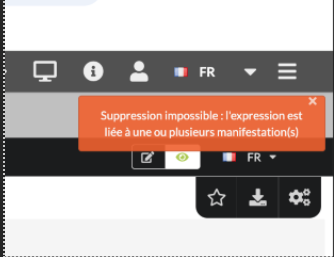
\includegraphics[width=0.7\textwidth]{images/terminologie.png} 
	
	\caption{Message de suppression d'une notice d'\gls{oeuvre}} 
	
	\label{figterminologie} 
	
\end{figure}

Cette proposition rejoint l’idée de supprimer la table œuvre cinématographique dans la gestion des masques alors que c’est la table œuvre/expression qui est couramment utilisée.  

Enfin, une confusion peut également s’installer entre les termes “œuvre liée” et “œuvre associée” dans les masques qui décrivent la \gls{manifestation} par exemple. Le terme d’œuvre liée pourrait être corrigé en “œuvre parente” pour que la nature du lien soit plus claire entre les deux entités.  

%\subsection{Conserver le niveau du FRBR en mode saisie sur les métas masques }
%
%Actuellement, lors de la configuration des méta-masques, les champs glissés et déposés dans le type de notice concernée perdent la mention du niveau FRBR auquel ils appartiennent. L’utilisateur n’a plus le moyen de savoir, une fois dans la notice, que tel champ appartient à tel niveau. Conserver la mention du niveau du FRBR sur les métas masques au sein de la saisie de la notice permettrait une meilleure compréhension et visibilité pour l’utilisateur. Ainsi, par exemple, dans une notice de \gls{manifestation}, le champ Titre afficherait : Œuvre – Titre.  

\section{Nouvelles fonctionnalités }

\subsection{Annotation de séquences sur un fichier vidéo numérique }

La table média actuelle permet seulement de visualiser une photo ou une vidéo, au clic sur la notice. Toutefois, il serait intéressant de développer une visionneuse spécifique à la vidéo qui permettrait non seulement de la visionner, mais également d’y placer des repères, des marqueurs, et de pouvoir l’annoter.  

Tout d’abord, deux possibilités de “séquençage” manuel seraient possibles :  

\begin{itemize}
	\item L’utilisateur saisit des repères temporels sur la vidéo sans la modifier. Ces repères sont reversés dans des champs prévus pour accueillir les “time codes” dans la notice de l’objet numérique. À l’ouverture du fichier numérique, les marqueurs laissés par l’utilisateur apparaissent, visibles sur la barre de défilement de la vidéo. L’utilisateur peut alors cliquer sur ces marqueurs pour naviguer au sein de la vidéo comme il le souhaite, et y voir les annotations associées.  
	
	\item L’utilisateur pourrait aussi vouloir segmenter le fichier vidéo en plusieurs séquences distinctes à partir de time codes précis. Dans ce cas-là, à la manière d’un logiciel de montage, l’utilisateur peut créer des cuts sur la vidéo et ainsi créer plusieurs fichiers numériques à partir de celle-ci, mais qui lui sont toujours liés. En effet, ces nouveaux objets, fragments du fichier vidéo d’origine, auraient leur propre notice de description mais resteraient rattachés à la notice principale, à la manière d’un ensemble.  
\end{itemize}

Cette nouvelle fonctionnalité permettrait d’apprécier l’hétérogénéité des collections, et s’avèrerait utile dans le cas, par exemple, de rushes documentaires non édités que l’utilisateur souhaiterait diviser par mots clés ou thématiques. La description des médias vidéo n’en serait que plus affinée et précisée.  

Par ailleurs, ce séquençage devra être effectué dans une optique d’annotation “sur” l’image, permettant ainsi d’associer des séquences plus précises à une description thématique. Concrètement, deux cas d’annotation sont possibles :  

\begin{itemize}
	\item L’utilisateur pourrait être capable de placer des tags sur des éléments de l’image (objets, personnes, éléments techniques, contenu...) et d’en décrire le contenu dans les champs prévus. La notice du média prévoit alors l’affichage d’une description par time codes, sur lesquels l’utilisateur peut cliquer pour accéder directement à l'image en question.  
	
	\item L’utilisateur peut également vouloir décrire une séquence dans sa globalité, à l’intérieur d’un time code précis. Dans ce cas, les champs sont saisis à partir d’un tag sur le time code, et non plus sur un élément précis de l’image.  L’affichage de la description dans la notice peut rester le même que le précédent.  
\end{itemize}


À l’ouverture du fichier vidéo, les annotations saisies apparaissent à droite de la visionneuse, et les times codes superposés à la barre de défilement de la vidéo.  

La description précise sur des séquences vidéo permettrait à la recherche d’être plus performante : l’utilisateur pourrait, en cherchant certains mots clés, tomber directement sur les séquences numériques associées, aux time codes correspondants. 

Il est intéressant de penser également à la mise en place d’une recherche par mots clés au sein du fichier numérique vidéo. La recherche d’un mot clé amène l’utilisateur à une séquence décrite par ce mot clé.   


\subsection{ \label{graphe}Mise en place d’une visualisation des liens entre entités du FRBR }

Cette idée s’inspire visuellement de la “balade intuitive” proposée par la bibliothèque Kandinsky dont voici un exemple :

\begin{figure}[htbp] 
	
	\centering 
	
	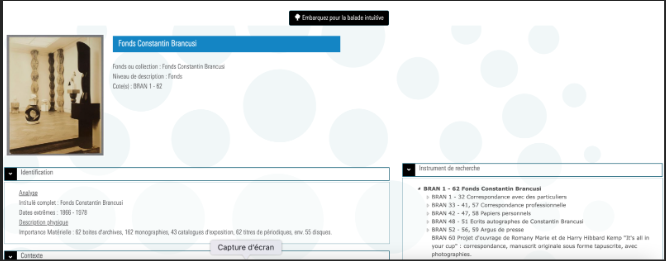
\includegraphics[width=1.0\textwidth]{images/kandinsky1.png} 
	
	\caption{Vue "balade intuitive" proposée par la bibliothèque Kandinsky \footcite{zotero-item-801}} 
	
	\label{figkandinsky1} 
	
\end{figure}

\begin{figure}[htbp] 
	
	\centering 
	
	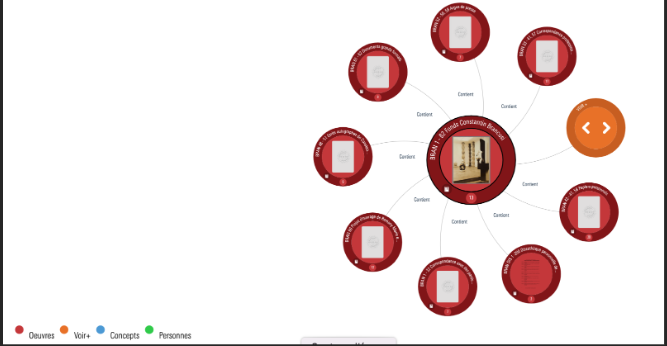
\includegraphics[width=1.0\textwidth]{images/kandinsky2.png} 
	
	\caption{Vue en graphe de la balade intuitive \footcite{zotero-item-801}} 
	
	\label{figkandinsky2} 
	
\end{figure}

Lorsque l’utilisateur ouvre S-Movies, ce sont les œuvres qui apparaissent sous la forme de résultats de recherche. Les liens avec d’autres notices (\gls{manifestation}s et \gls{item}s) n’apparaissent pas à première vue. Il faut ouvrir une notice pour voir la liste des entités qui y sont liées, si toutefois ces liens sont configurés dans le menu de la notice. Or, la visualisation de liens entre les entités d’une collection est primordiale dans la logique d’une structuration selon le modèle FRBR. Pouvoir avoir un aperçu de ces liens pourrait améliorer la compréhension de la hiérarchie entre les niveaux du FRBR et leur délimitation, et ainsi améliorer les pratiques de saisie selon les cas d’indexation. De plus, visualiser rapidement les liens entre entités permettrait d’identifier les incohérences et les erreurs de données plus facilement, comme par exemple, des éléments vides ou isolés. 

Les entités principales du FRBR étant au nombre de trois, la représentation choisie pourrait être celle d’une représentation en graphes de connaissances, modélisant ainsi les relations entre entités. Cette représentation s’appuie sur le modèle de graphe RDF (sujet-prédicat-objet) qui permet également l’interopérabilité des données.  

Pour penser la place que pourrait prendre cette visualisation des liens dans l’application, il faut se poser les questions suivantes : quel niveau du FRBR les utilisateurs préfèrent-ils visualiser ? Dans quel contexte ? Autrement dit, il faut se demander quel niveau de granularité choisir pour mettre en place cette visualisation et à quel endroit de l’application. 

Puisque la page d’accueil de l’espace de travail S-Movies présente les œuvres, la représentation en graphe pourrait dans un premier temps permettre de visualiser les œuvres présentes dans la collection.  

Le premier niveau permettrait donc à l’utilisateur de visualiser la liste des œuvres préservées sous formes de cercles, plus ou moins gros selon le nombre de sous-niveaux qu’elles contiennent. Ainsi, une œuvre qui contiendrait deux \gls{variante}s, quatre \gls{manifestation}s, 12 \gls{item}s sera plus grande qu’une \gls{oeuvre} qui contient 1 \gls{manifestation} et 1 \gls{item}.  

Au clic sur l’\gls{oeuvre}, le détail de ses relations avec des sous-éléments apparait : \gls{variante}s, \gls{manifestation}s, \gls{item}s.  

Ce mode d’affichage pourrait être disponible de la même manière que les modes d’affichage déjà présents dans l’application. Il faudrait ajouter un mode d’affichage en “graphe”. 

\begin{figure}[htbp] 
	
	\centering 
	
	
\includegraphics[width=0.6\textwidth]{images/vue.png} 
	
	\caption{Modes d'affichage disponibles dans l'application} 
	
	\label{figvues} 
	
\end{figure}

Ce mode d’affichage, établit au niveau des tables, pourrait également être disponible au niveau des notices. Par exemple dans une notice d’\gls{item}, un onglet de menu pourrait être configurable pour faire apparaitre, en graphe, les relations de l’\gls{item} avec les niveaux parents du \gls{FRBR}.   

Il serait intéressant d’intégrer à ces visualisations en graphes les médias, d’autant plus dans le cas de la mise en place d’une segmentation vidéo, pour pouvoir visualiser les différents segments reliés à l’\gls{item}.  

Concrètement, le parcours utilisateur de cet affichage serait le suivant :   
\begin{itemize}
	\item Que ce soit depuis une table ou depuis une notice, l’utilisateur clique sur le mode d’affichage en graphe  
	
	\item Les entités concernées s’affichent sous la forme de cercles, proportionnels aux nombres de liens qu’ils entretiennent avec les autres niveaux du \gls{FRBR}. Les cercles comportent des informations minimales selon le niveau : le titre et la date pour les œuvres, le titre le format et la date pour les \gls{manifestation}s, le titre, le format, la date et l’identifiant pour l’\gls{item}. 
	
	\item Une légende s’affiche en bas de l’écran avec un code couleur pour chaque entité, et le nombre d’entités présentes.  
	
	\item Au clic de l’utilisateur sur l’un des cercles, le détail des relations de l’entité avec d’autres entités s’ouvre en mode graphe. Le résumé de la notice s’affiche en barre latérale sur le côté.  
	
	\item Au clic sur une entité liée, le graphe se reforme et l’entité choisie devient le centre du graphe.  
\end{itemize}


On pourrait également ajouter au graphe les lieux et les personnes (intervenants) liés à chaque entité du \gls{FRBR}. 



\chapter{\label{annexe_B}Spécification fonctionnelle : Recherche en langage naturel à l’appui de l’intelligence artificielle } 
\titreEntete{Specification fonctionnelle}

Cette seconde annexe, présente une spécification fonctionnelle pour la mise en place d'un outil de recherche en langage naturel, fondé sur l'intelligence artificielle, rédigée à la demande de Skinsoft dans le cadre de notre stage. Cet outil est actuellement en cours de développement. L'implémentation de la recherche en langage naturel a fait l'objet de recherches et de réflexions parallèles à celles de la segmentation et de l'indexation automatisées. Le document est structuré en deux parties : les principes d'usage théoriques, la spécification fonctionnelle détaillée à l'appui de maquettes visuelles. 

Cette spécification a été rédigée conjointement avec Florian Martin, également stagiaire chez Skinsoft.
Réduite pour les besoins de notre étude, cette annexe fait en réalité partie d'une spécification plus large rendue avec ce mémoire comme livrable technique. 

\section{Le besoin utilisateur}

L’application doit proposer un mode de recherche alternatif à la recherche simple, basé sur l’intelligence artificielle. Cela doit permettre de questionner l’application en langage naturel dans un double objectif :  

Rendre chaque table interrogeable sans utilisation de vocabulaire contrôlé ou de la recherche avancée : une simple phrase suffit 

Par exemple : 

\begin{itemize}
	\item “Tous les films réalisés par David Lynch en 1987” 
	
	\item “Tous les films numériques” 
	
	\item “Toutes les photos au format dng” 
\end{itemize} 

Agir comme un générateur de requête exécutable par l’utilisateur sur la table interrogée ET la recherche fédérée.  

\section{Principes d'usage}

\subsection{Mode de "recherche augmentée" alternatif \label{infobulle}}

Dans les outils de recherche, à côté de la barre de recherche je clique sur le bouton de recherche augmentée. La barre de recherche passe de la fonctionnalité “recherche simple” à la “recherche augmentée” : on peut interroger la table en question à l’aide de phrases.  

Il y a une distinction visuelle établie dès le clic :  

\begin{itemize}
	\item Le fond du bouton se colorie selon la couleur de l’interface définie dans la notice d’établissement. Fonctionnement actuel des autres boutons 
	
	\item Apparition d’un symbole warning dans la barre de recherche, à son extrémité droite. Au survol avec la souris, une infobulle s’ouvre avec le message : “Recherche augmentée activée, vous utilisez l’intelligence artificielle. Fonctionnalité limitée à l’usage des données existantes.”  
\end{itemize}


Changement du message inscrit dans la barre de recherche :  

\begin{itemize}
	\item Recherche simple : “Recherche” 

	\item Recherche augmentée : “Interrogez-moi”
\end{itemize}  

\subsection{Gestions des erreurs}

Deux logiques : 

\begin{itemize}
	\item La possibilité pour le processus d’indiquer qu’il ne comprend pas la requête utilisateur afin d’éviter la création d’une requête erronée. 
	\item La possibilité pour l’utilisateur de signaler un problème. 

\end{itemize}

En cas d’incompréhension de la requête utilisateur et d’incertitude sur la requête à générer. La fonctionnalité doit :  

\begin{itemize}
	\item Ne pas lancer la requête car il n’est pas certain.  

	\item Identifier le point bloquant  

	\item Signaler l’erreur par un code couleur : 
	
	\subitem Le mot posant un problème est surligné en rouge lorsque incompréhension totale. 
	
	\subitem Le mot pose un problème est surligné en orange lorsqu’il y a une incertitude sur le sens. 
	
\end{itemize}


L’utilisateur doit pouvoir écrire dans la barre de recherche un complément à la requête d’origine. 

\begin{itemize}
	\item Le complément s’envoie au processus comme une requête classique. C’est l’interprétation qui change.  

	\item S'il y a toujours une erreur, on revient à l’étape précédente jusqu’à résolution de l’erreur.  

	\item Si l’utilisateur tombe dans une boucle infinie et décide d’arrêter le traitement, l’absence d’activité dans la barre de recherche dans les 30 secondes met fin au processus.  

	\item Si le complément amène à résoudre l’erreur, le processus suit son cours. 
\end{itemize}



En cas d’une requête générée mais invalide selon l’utilisateur, ce dernier peut la reporter afin que le modèle enregistre l’incident, comprenne l’erreur et s’affine. 

À côté du résumé se trouve un bouton “Reporter une erreur”  

Au clic sur le bouton, ouverture d’un formulaire afin de reporter une erreur. S’ouvre comme une notice. 

Quatre champs sont affichés :  

\begin{itemize}
	\item Champ Titre du rapport : l’utilisateur saisi un titre pour le rapport d’erreur. Permet de le rendre traçable. 

	\item Champ requêtes : rempli automatiquement, il contient la requête utilisateur (la phrase de départ) + le résumé de la recherche générée par IA. Non visible par l’utilisateur, y figure aussi la requête ElasticSearch générée.  

	\item Champ date : rempli automatiquement avec le jour de requêtage 

	\item Champ description : l’utilisateur explique pourquoi cela ne lui convient pas et ce qu’il attendait.  
\end{itemize}



Deux boutons sont disponibles :  

\begin{itemize}
	\item “Envoyer” : 
	\subitem Envoie le rapport d’incident au LLM, l’historise et l’intègre dans une base de données pour entraînement. 

	\subitem Génère une notification verte à l’endroit habituel : “Rapport d’erreur envoyé et enregistré”. 

	\item “Annuler” : Annule l’opération en cours. 

	\subitem Génère une notification orange à l’endroit habituel : “Rapport d’erreur annulé”. 
\end{itemize}



\section{Fonctionnalité détaillée}

\subsection{Infobulle}

Au survol de la souris, le symbole affiche une infobulle contenant un court message qui informe l’utilisateur de l’utilité de la recherche activée. Le symbole est affiché en tout temps lorsque la recherche augmentée est activée. 

\begin{figure}[htbp] 
	
	\centering 
	
	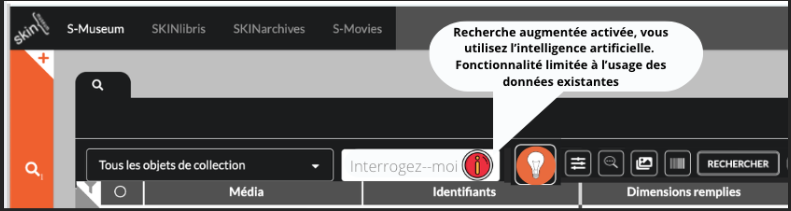
\includegraphics[width=1.0\textwidth]{images/infobulle.png} 
	
	\caption{Infobulle d'activation} 
	
	\label{figinfobulle} 
	
\end{figure}

\subsection{Requête mal formulée ou incertaine}

Si la requête de l’utilisateur est mal formulée ou incorrecte, empêchant la recherche augmentée d’être lancée, deux options sont possibles.  

Si l’outil est incertain quant à l’interprétation d’un terme utilisé dans la requête, celui-ci est surligné en couleur orange :  

\begin{figure}[htbp] 
	
	\centering 
	
	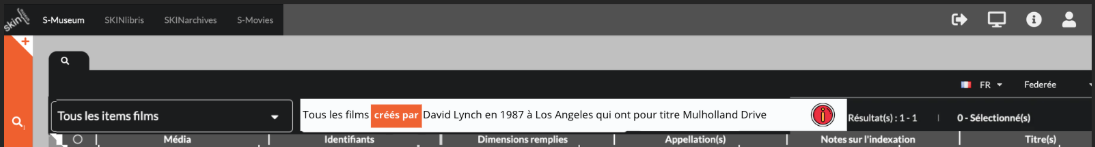
\includegraphics[width=1.0\textwidth]{images/annexe1.png} 
	
	\caption{Incertitude quant au terme utilisé} 
	
	\label{figincertitude} 
	
\end{figure}

Si l’outil ne comprend pas la requête, parce qu’elle est incohérente ou inadaptée, celle-ci est surlignée en rouge :  

\begin{figure}[htbp] 
	
	\centering 
	
	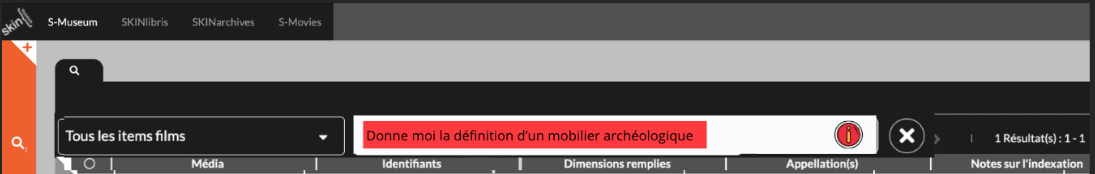
\includegraphics[width=1.0\textwidth]{images/annexe2.png} 
	
	\caption{Incohérence du terme utilisé} 
	
	\label{figIncoherence} 
	
\end{figure}

\subsection{Résultats de recherche invalides :}

Si les résultats de recherche retournés par la recherche augmentée sont erronés selon l’utilisateur, et ne correspondent pas à la requête qui a été formulée, il peut signaler l’incident dans un formulaire prévu à cet effet, via un bouton “reporter un problème” dans l’onglet de résumé : 

\begin{figure}[htbp] 
	
	\centering 
	
	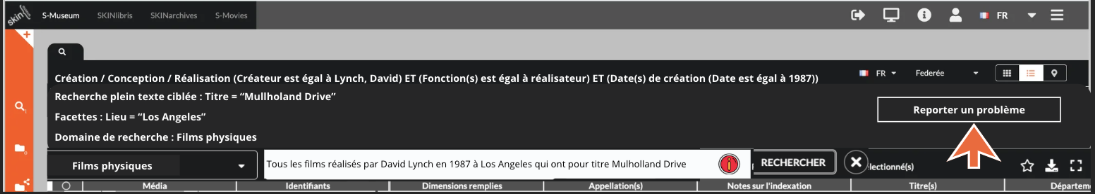
\includegraphics[width=1.0\textwidth]{images/annexe3.png} 
	
	\caption{Reporter un problème} 
	
	\label{figReporteunPb} 
	
\end{figure}

Au clic sur ce bouton, un formulaire s’ouvre sous la forme d’une notice que l’utilisateur peut remplir pour décrire le problème détecté. Les champs “date” (format calendaire) et “requête effectuée” sont automatiquement remplis :  

\begin{figure}[htbp] 
	
	\centering 
	
	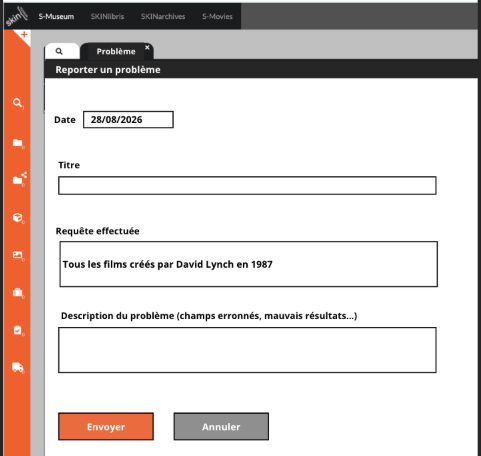
\includegraphics[width=1.0\textwidth]{images/annexe4.png} 
	
	\caption{Formulaire d'erreur} 
	
	\label{figFormulaire} 
	
\end{figure}

Au clic sur “envoyer”, un message de validation apparait :  

\begin{figure}[htbp] 
	
	\centering 
	
	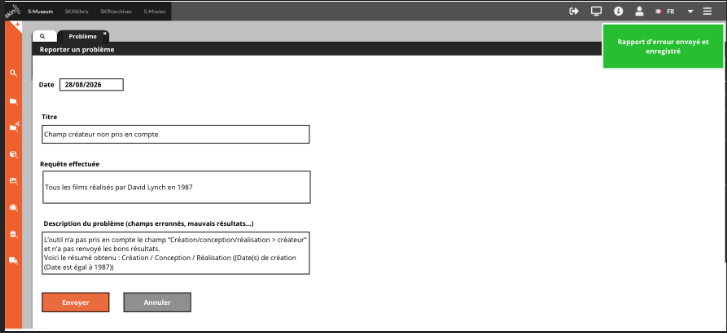
\includegraphics[width=1.0\textwidth]{images/annexe5.png} 
	
	\caption{Message de validation} 
	
	\label{figValidation} 
	
\end{figure}